\documentclass{article}

\usepackage[final]{neurips_2023}
\usepackage[utf8]{inputenc}
\usepackage[T1]{fontenc}
\usepackage{hyperref}
\usepackage{url}
\usepackage{booktabs}
\usepackage{amsfonts}
\usepackage{nicefrac}
\usepackage{microtype}
\usepackage{xcolor}
\usepackage{graphicx}
\graphicspath{{../repro/}}
\usepackage{subcaption}
\usepackage{multirow}
\usepackage{siunitx}
\usepackage{enumitem}
\usepackage{array}
\usepackage{tabularx}
\usepackage{placeins}
\usepackage{float}

\title{\datasetname{}: \datasetfull{} Segmentation Benchmark}

\author{%
  Anonymous Authors\\
  Anonymous Institution\\
  \texttt{anonymous@anonymous.edu}
}

\newcommand{\datasetname}{AMAM-128}
\newcommand{\datasetfull}{Annotated Metallic Alloys Microstructures}
\newcommand{\paircount}{128}
\newcommand{\subsetcount}{6}
\newcommand{\tablefontsize}{\small}

\begin{document}

\maketitle

\begin{abstract}
Metallography segmentation remains difficult because phase semantics and image
statistics shift across materials, processing conditions, and magnification
regimes. Existing datasets are often strong in one regime but limited for
cross-regime benchmarking. We present \datasetfull{} (\datasetname{}), a strict
pair-only benchmark with \paircount{} image--mask tuples across \subsetcount{}
curated subsets. \datasetname{} spans two material families, four processing
conditions, and six subset-specific regimes covering four nominal
magnifications (x5/x10/x20/x50) while preserving subset-native phase semantics.
We report a unified 45-method campaign (10 classical, 29 supervised deep, 6
foundation/edge) on the same paired corpus with common subset-macro reporting
and explicitly disclosed track-specific label handling.
The highest displayed central estimate is the fixed-seed RF score of 0.630
macro mIoU, evaluated with the classical track's per-image label-permutation
alignment, leaving a 0.370 gap to perfect overlap; the highest displayed
foundation/edge score is 0.437 under the same form of alignment. Supervised deep scores
are evaluated without this alignment, so the cross-track ordering is
descriptive rather than a strict semantic leaderboard.
The 29 supervised models are evaluated in five clean retraining runs (seeds
17--21), and subset-macro mIoU is reported as the five-run mean $\pm$ sample
standard deviation. The median per-model sample standard deviation
($s=0.0318$ macro mIoU) is approximately 7.2 times the median adjacent-model
gap in the mean-ranked table ($0.00443$). The results should therefore be read
descriptively rather than as identifying a unique best supervised model or a
stable fine-grained ordering. Because the executed seed sweep varies both model-side stochasticity
and seeded label-decoding operations, the spread represents end-to-end run
variability rather than pure training noise. These results indicate
substantial unsolved headroom and motivate methods that improve regime
robustness rather than single-slice tuning. \datasetname{} is intended as a
controlled benchmark-comparison resource, not an out-of-sample generalization
benchmark. Benchmark repository (interactive explorer and downloadable
artifacts): \url{https://github.com/Scientific-Computing-Lab/AMAM}.
\end{abstract}

\section{Introduction}
Automated microstructure segmentation is foundational for quantitative metallography, yet benchmark methodology remains underdeveloped. The main challenge is not only annotation count: alloy family, process state, magnification, and imaging artifacts all change the segmentation regime. Benchmarks that flatten these shifts into one pooled setting can overstate progress.

Prior resources enabled important progress, including UHCS-focused datasets, broader materials-segmentation efforts, and metallography-specific pipelines~\citep{decost2017uhcsdb,decost2019high,luengo2022tutorial,rusanovsky2020mlography,rusanovsky2022end}. However, many public settings remain narrow in at least one benchmark-critical axis: material-family breadth, cross-scale coverage, artifact-stress auditing, or strict pair-only inclusion. Recent foundation segmentation systems also transfer well in natural imagery but remain fragile on texture-heavy metallography boundaries and artifact confounds~\citep{kirillov2023segment,ji2023segment,rusanovsky2025texturesam,cohen2024mlographypp}. A compact landscape comparison is given in Appendix~\ref{app:landscape} (Table~\ref{tab:benchmark_landscape}), with broader related-work context in Appendix~\ref{app:related}.

\datasetfull{} (\datasetname{}) addresses this gap with a strict rule: only
image--mask pairs are included. The release contains \paircount{} paired
tuples, with no unpaired samples in evaluation. It spans two material families,
four process conditions, and six subset-specific regimes covering four nominal
magnifications (x5/x10/x20/x50) while preserving subset-native phase semantics.
In the campaign reported here, all model families use the same paired corpus
and subset-macro aggregation, with track-specific prediction-to-label handling
reported explicitly. The supervised deep models
and the RF/SVM classical baselines are fit on that same paired set, so their
scores measure in-corpus fit rather than transfer. The remaining classical
procedures do not use AMAM masks to fit supervised parameters, although
several fit clusters to each input image; pretrained foundation/edge networks
are used without AMAM parameter updates. Their predicted segment identifiers
are matched to reference classes during evaluation. Because the release is intentionally compact, we frame this
as a controlled benchmarking audit rather than a large-corpus training
benchmark. The strength of this dataset also lies in its inclusion of
non-ideal, real-world images where etching may be inconsistent, surface
artifacts like stains and scratches are present, and features such as mounting
boundaries, specimen edges, or micro-hardness indentations are visible within
the frame.

Our contribution is benchmark-centric: (i) a strict pair-only release
specification, (ii) a multi-regime design that jointly captures material,
process, scale, and artifact stressors, (iii) a 45-method audit (10 classical,
29 supervised deep, 6 foundation/edge) under one full-pair campaign framework,
with persistent headroom (highest displayed central estimate 0.630, from the
fixed-seed RF pixel-feature baseline), and (iv) a multi-seed reproducibility
protocol that quantifies
end-to-end run variability in the supervised pipeline and reports per-model
score and rank spread, allowing reported differences to be compared with the
variability of the executed protocol. This makes the benchmarking gap
measurable rather than anecdotal.

\section{The AMAM-128 Benchmark}
\textbf{Benchmark design.} \datasetname{} includes six subsets: 4130 steel
(x10/x20), 5884 armor steel (x5/x10/x20/x50), 418 printed 17-4 PH (x5 and
x20), and 6280 gray cast iron (x10 and x20). The six subsets define 13
subset-local class slots corresponding to nine distinct phase names; label
spaces remain subset-specific to avoid invalid class merging across materially
different phase taxonomies. Figure~\ref{fig:workflow} summarizes the
annotation/refinement pipeline used to construct the final paired release.

\begin{figure}[t]
    \centering
    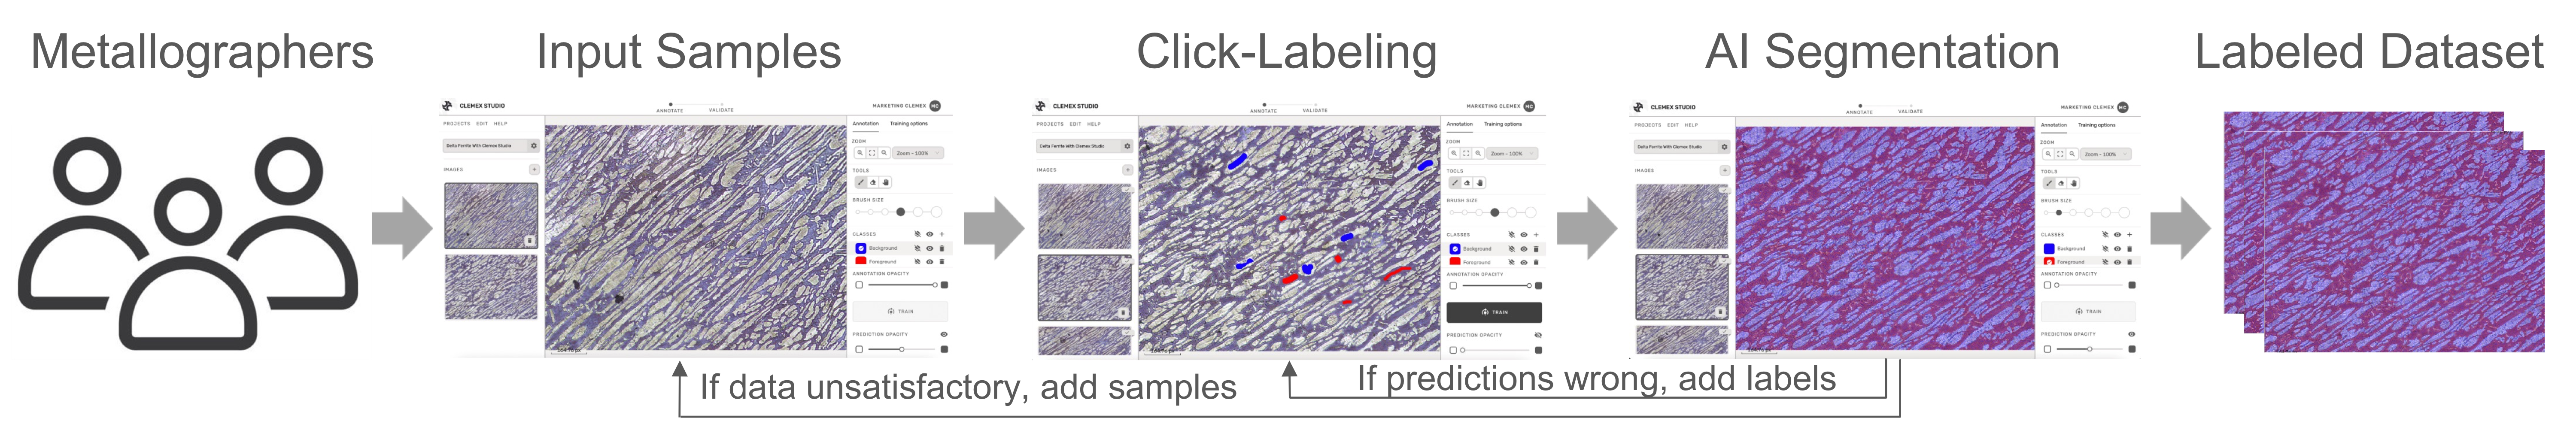
\includegraphics[width=\linewidth,trim=25 20 45 60,clip]{../assets/images/amam-workflow.png}
    \caption{AMAM annotation and refinement workflow. From left to right,
    domain experts provide representative micrographs, create sparse
    click-level supervision, run model-assisted dense
    segmentation\protect\footnotemark, and iteratively review and correct
    predictions. Accepted masks are then frozen into the paired benchmark
    release.}
    \label{fig:workflow}
\end{figure}
\footnotetext{Model-assisted segmentation in this workflow used Clemex Studio AI tooling; product overview: \url{https://clemex.com/clemex-studio-easy-segmentation/}. A benchmark-facing use of this studio-assisted paradigm for grain-size-oriented metallography appears in MLOGraphy++~\citep{cohen2024mlographypp}.}

\textbf{Why the heterogeneous design matters.} \datasetname{} is intentionally
compact but heterogeneous: it combines ferrite/pearlite separation,
dendrite/interdendritic structure, graphite-flake segmentation, and
printed-alloy grain patterns in one suite. This design exposes multiple
in-corpus regimes instead of collapsing them into one pooled setting.

\textbf{Evaluation tracks.} The executed campaign reports within-subset
performance under one full-pair campaign framework. For future extensions, we
recommend adding two explicit OOD tracks: (i) cross-material transfer after
defining a compatible target label space and (ii) within-material
magnification-shift transfer between subsets with compatible labels.
Reporting should prioritize subset-macro mIoU (Dice/Pixel Accuracy secondary)
to prevent large subsets from dominating scores. Under the executed CUDA
configuration, clean supervised retraining runs were not assumed to be
bit-identical. The supervised track is therefore evaluated in five clean
end-to-end runs using seeds 17--21, and its primary score is reported as the
five-run mean $\pm$ sample standard deviation (median per-model $s=0.0318$
macro mIoU). This spread includes both model-side stochasticity and seeded
label-decoding operations.


\textbf{Release accounting and category audit.} Verified release statistics
are reported in Table~\ref{tab:globalstats}, representative originals/masks
are shown in Figure~\ref{fig:main_diversity_pairs}, and expanded aligned
image-level evidence appears in Tables~\ref{tab:rep_visual_diversity}
and~\ref{tab:rep_visual_diversity_part2}. Complementary release accounting
appears in Appendix~\ref{app:release}, Appendix~\ref{app:subset}, and
Appendix~\ref{app:ood}; expanded visual audit framing is in
Appendix~\ref{app:visual}; and release-metadata annotation notes are summarized
in Appendix~\ref{app:annotationnotes} (Table~\ref{tab:annotation_notes}).

\begin{figure}[t]
    \centering
    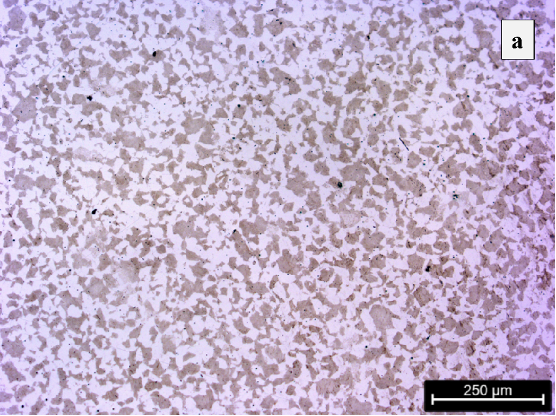
\includegraphics[width=0.24\linewidth]{../assets/images/4130-steel-original.png}
    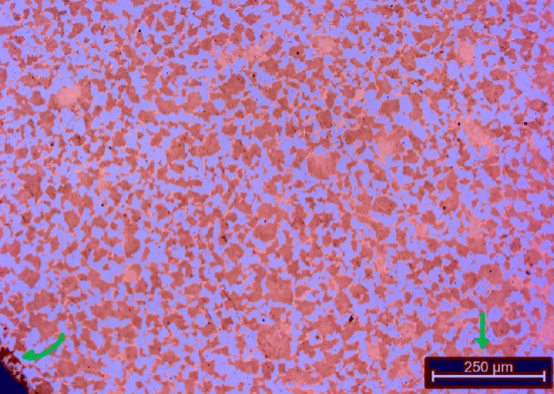
\includegraphics[width=0.24\linewidth]{../assets/images/4130-steel-labeled.png}
    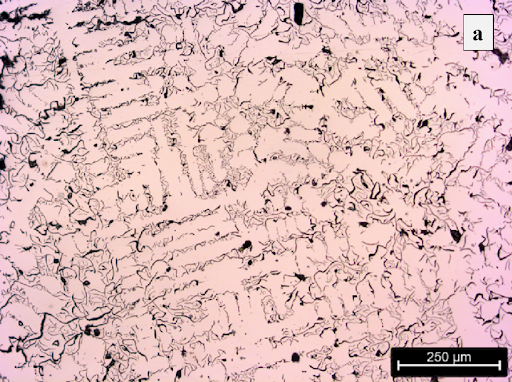
\includegraphics[width=0.24\linewidth]{../assets/images/6280-cast-iron-low-original.jpg}
    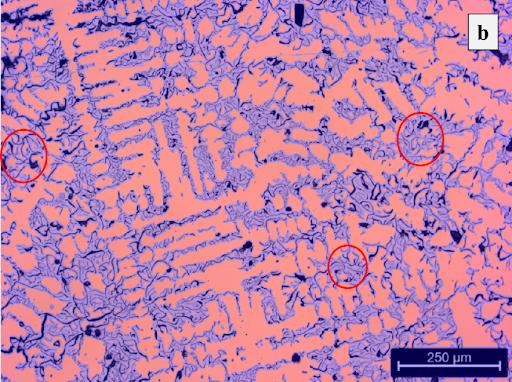
\includegraphics[width=0.24\linewidth]{../assets/images/6280-cast-iron-low-labeled.jpg}
    \\
    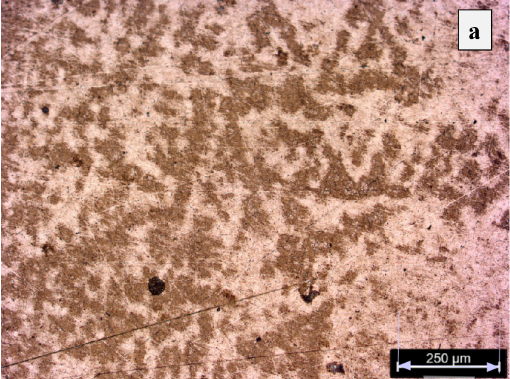
\includegraphics[width=0.24\linewidth]{../assets/images/5884-armor-steel-original.jpg}
    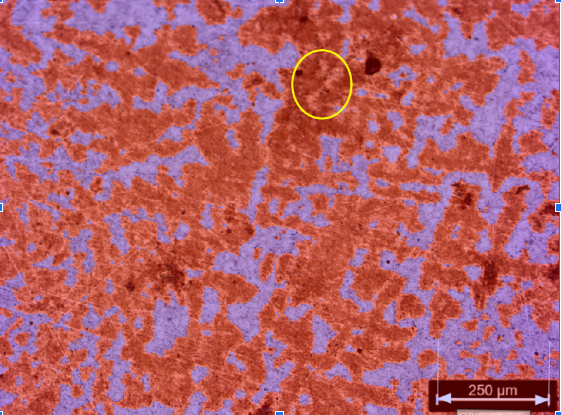
\includegraphics[width=0.24\linewidth]{../assets/images/5884-armor-steel-labeled.jpg}
    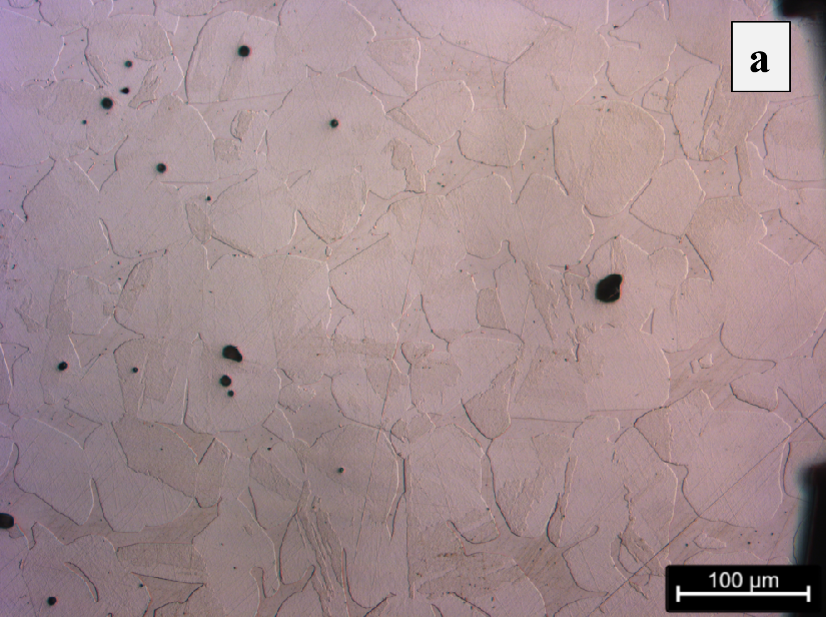
\includegraphics[width=0.24\linewidth]{../assets/images/418-17-4ph-x5-original.jpg}
    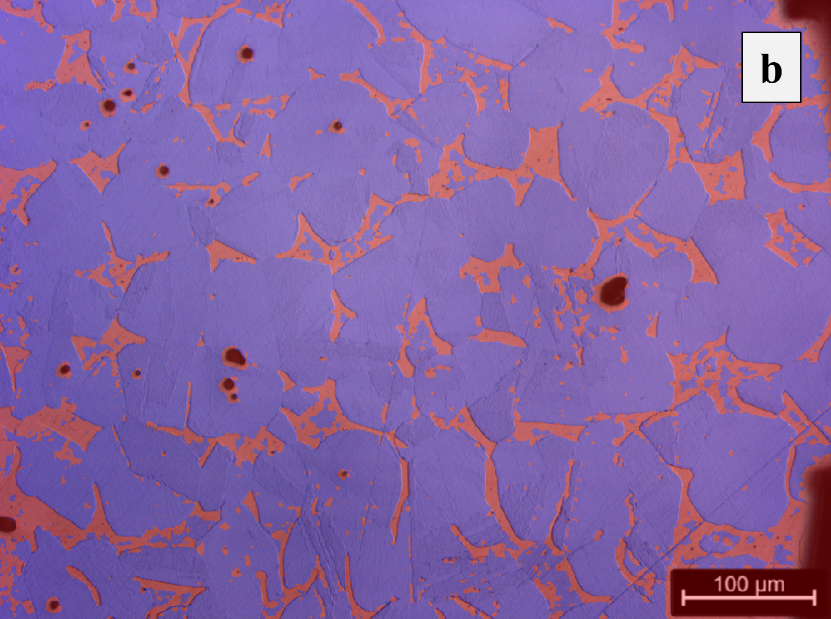
\includegraphics[width=0.24\linewidth]{../assets/images/418-17-4ph-x5-labeled.jpg}
    \caption{Representative AMAM-128 image--mask pairs from four distinct regimes. Top row: 4130 steel (x10/x20 family) and 6280 cast iron x10 (original/mask pairs). Bottom row: 5884 armor steel (x5/x10/x20/x50 family) and printed 17-4 PH x5 (original/mask pairs). The diversity in texture scale, boundary sharpness, and phase morphology illustrates why regime-aware benchmarking is necessary.}
    \label{fig:main_diversity_pairs}
\end{figure}

\section{Results Over Current Models}
\textbf{Benchmarking setup.} We evaluate three tracks: (i) classical (10),
(ii) supervised deep (29, general-purpose + metallography-oriented), and (iii)
foundation/edge add-ons (6). All use strict pair-only inclusion and
subset-macro reporting. Classical and foundation/edge entries use the fixed
seed-17 protocol, whereas supervised deep mIoU values are aggregated over five
clean runs using seeds 17--21. The RF/SVM classical baselines and supervised
deep models are fit on all \paircount{} tuples and evaluated on those same
tuples; the other classical methods use no AMAM mask supervision (although
several fit clusters per image), and foundation/edge add-ons use no AMAM
parameter updates. Every classical and
foundation/edge prediction is evaluated using the known subset phase count and
per-image Hungarian label-permutation alignment. Deep predictions are instead
scored directly after restricting logits to the known subset-valid classes
(protocol details in Appendix~\ref{app:repro}).\footnote{Reproduction
package for this 45-method audit (run scripts, protocol files,
checkpoint/source manifest, and consistency audit):
\url{https://github.com/Scientific-Computing-Lab/AMAM/tree/main/repro}.}
Absolute scores should therefore be interpreted as in-corpus diagnostics. The
campaign provides a controlled, descriptive comparison on a shared corpus, but
does not estimate out-of-sample generalization and does not erase the
track-specific label handling described in Appendix~\ref{app:repro}.



\textbf{Main empirical evidence.} Figure~\ref{fig:gap_overview} summarizes all
45 methods. The highest displayed central estimate is the fixed-seed RF score
of 0.630 mIoU, and the median across the 45 displayed centers is 0.530.
Group-highest entries are RF (classical, 0.630), U-Net
(EfficientNet-B0) (deep-general, $0.594\pm0.013$), Metal-MAnet RGB+Sobel
(EfficientNet-B0) (deep metallography, $0.610\pm0.020$), and SAM ViT-Base
(foundation/edge, 0.437).

\begin{figure}[t]
    \centering
    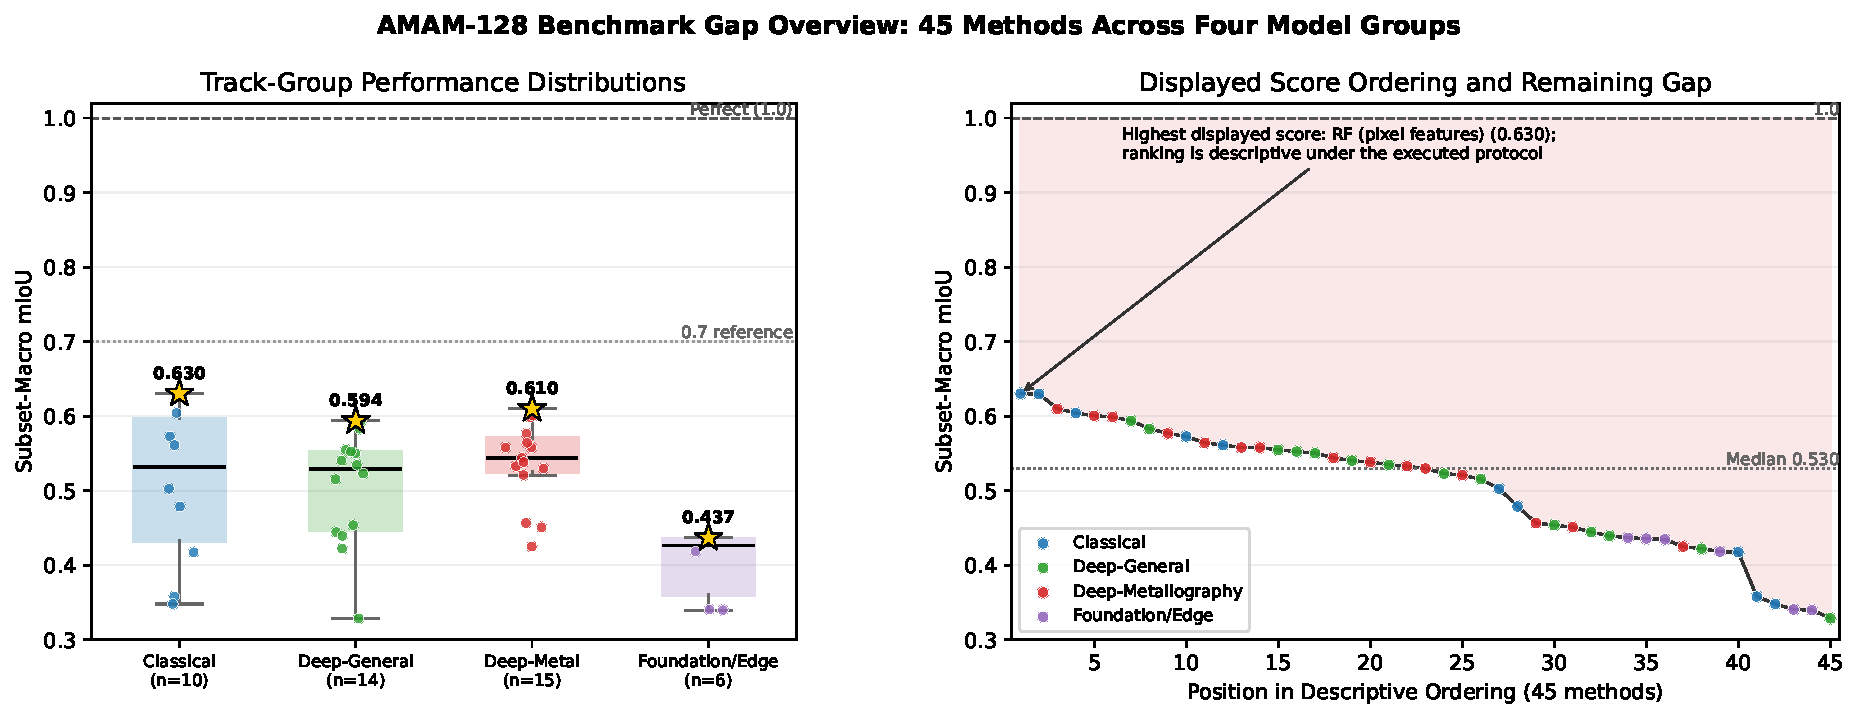
\includegraphics[width=\linewidth]{../repro/figures/benchmark-gap-overview.pdf}
    \caption{
    Cross-family benchmark gap over all 45 tested methods (10 classical, 14
    deep-general, 15 deep-metallography, 6 foundation/edge). Deep points use
    five-run mean mIoU; classical and foundation/edge points use fixed seed-17
    estimates. Left: per-group distributions with highest-in-group markers.
    Right: descriptive ordering of the displayed centers and gap to perfect
    overlap (1.0). Full per-method metrics and deep run-to-run spread are
    reported in Table~\ref{tab:benchmark-model-results}.
    }
    \label{fig:gap_overview}
\end{figure}

\textbf{Cross-family findings.} No family saturates this benchmark.
Metallography-aware deep variants approach the highest classical scores, and
prompt-free foundation transfer remains lower under the displayed metrics.
These cross-track differences are descriptive rather than a strict semantic
leaderboard because classical/foundation predictions and supervised deep
predictions use different label-handling conventions (Appendix~\ref{app:repro}).

\textbf{Observed failure patterns.} Qualitative inspection of representative
predictions suggests that errors often occur near ferrite/pearlite and
dendrite/interdendrite boundaries, in sparse artifact regions
(pores/scratches), and in reflective high-contrast zones. Released per-subset
metrics also show substantial within-corpus performance heterogeneity. Because
no held-out regime was evaluated, these observations should not be interpreted
as evidence about cross-regime transfer.


\begin{table}[H]
    \centering
    \footnotesize
    \setlength{\tabcolsep}{3pt}
    \renewcommand{\arraystretch}{0.95}
    \caption{Benchmark model results on \datasetname{} (45 methods, macro over
subsets) under the full-pair campaign protocol. Highest displayed value per metric
over all methods is bold; displayed values are rounded to three decimals and
ties are broken at full precision. Supervised deep mIoU values are five-run
means $\pm$ sample standard deviations over clean runs using seeds 17--21;
their Dice and Pixel Accuracy values are seed-17 point estimates. The standard
deviation measures observed end-to-end run variability and is not a confidence
interval for dataset-sampling uncertainty. Classical and foundation/edge
values are fixed seed-17 point estimates and have no reported cross-seed
uncertainty. Classical/foundation entries use per-image Hungarian label
alignment; deep entries do not, so bolding is descriptive rather than evidence
of a like-for-like semantic ranking.
}
    \label{tab:benchmark-model-results}
    \begin{tabularx}{\linewidth}{>{\raggedright\arraybackslash}Xrrr}
        \toprule
        Model & mIoU & Dice & Pixel Acc \\
        \midrule
        \multicolumn{4}{l}{\textbf{Classical (10)}} \\
        RF (pixel features)~\citep{breiman2001random} & \textbf{0.630} & \textbf{0.742} & 0.817 \\
        Linear SVM (pixel features)~\citep{cortes1995support} & 0.630 & 0.739 & 0.832 \\
        GMM-RGB~\citep{bishop2006pattern} & 0.604 & 0.714 & 0.818 \\
        Gabor-KMeans~\citep{daugman1985uncertainty,lloyd1982least} & 0.573 & 0.691 & 0.791 \\
        KMeans-RGB~\citep{lloyd1982least} & 0.561 & 0.667 & 0.791 \\
        SLIC+KMeans~\citep{achanta2012slic,lloyd1982least} & 0.503 & 0.613 & 0.756 \\
        Felzenszwalb-GMM~\citep{felzenszwalb2004efficient,bishop2006pattern} & 0.479 & 0.584 & 0.748 \\
        LBP+KMeans~\citep{ojala2002multiresolution,lloyd1982least} & 0.417 & 0.558 & 0.615 \\
        Sobel+Watershed~\citep{canny1986computational,beucher1979use} & 0.358 & 0.499 & 0.571 \\
        Canny+Watershed~\citep{canny1986computational,beucher1979use} & 0.348 & 0.437 & 0.657 \\
        \midrule
        \multicolumn{4}{l}{\textbf{Supervised Deep --- General (14)}} \\
        U-Net (EfficientNet-B0)~\citep{ronneberger2015u,tan2019efficientnet} & 0.594 {\tiny$\pm$0.013} & 0.706 & 0.806 \\
        DeepLabV3+ (EfficientNet-B0)~\citep{chen2018encoder,tan2019efficientnet} & 0.583 {\tiny$\pm$0.006} & 0.706 & 0.821 \\
        U-Net++ (ResNet34)~\citep{zhou2018unetpp,he2016deep} & 0.555 {\tiny$\pm$0.031} & 0.710 & 0.806 \\
        SegFormer (MiT-B2)~\citep{xie2021segformer} & 0.553 {\tiny$\pm$0.038} & 0.609 & 0.727 \\
        U-Net (ResNet34)~\citep{ronneberger2015u,he2016deep} & 0.550 {\tiny$\pm$0.027} & 0.679 & 0.768 \\
        DeepLabV3+ (ResNet34)~\citep{chen2018encoder,he2016deep} & 0.540 {\tiny$\pm$0.053} & 0.673 & 0.776 \\
        SegFormer (MiT-B0)~\citep{xie2021segformer} & 0.535 {\tiny$\pm$0.036} & 0.709 & 0.807 \\
        MAnet (ResNet34)~\citep{fan2020manet,he2016deep} & 0.523 {\tiny$\pm$0.042} & 0.673 & 0.762 \\
        LinkNet (ResNet34)~\citep{chaurasia2017linknet,he2016deep} & 0.515 {\tiny$\pm$0.037} & 0.591 & 0.726 \\
        UPerNet (MiT-B2)~\citep{xiao2018upernet,xie2021segformer} & 0.454 {\tiny$\pm$0.031} & 0.499 & 0.622 \\
        PSPNet (ResNet34)~\citep{zhao2017pspnet,he2016deep} & 0.445 {\tiny$\pm$0.012} & 0.524 & 0.705 \\
        UPerNet (MiT-B0)~\citep{xiao2018upernet,xie2021segformer} & 0.439 {\tiny$\pm$0.012} & 0.449 & 0.561 \\
        FPN (ResNet34)~\citep{lin2017fpn,he2016deep} & 0.422 {\tiny$\pm$0.051} & 0.577 & 0.707 \\
        DeepLabV3 (ResNet34)~\citep{chen2017rethinking,he2016deep} & 0.329 {\tiny$\pm$0.041} & 0.372 & 0.651 \\
        \midrule
        \multicolumn{4}{l}{\textbf{Supervised Deep --- Metallography-Oriented (15)}} \\
        Metal-MAnet RGB+Sobel (EfficientNet-B0)~\citep{fan2020manet,tan2019efficientnet} & 0.610 {\tiny$\pm$0.020} & 0.720 & 0.826 \\
        Metal-U-Net++ CLAHE (EfficientNet-B0)~\citep{zhou2018unetpp,tan2019efficientnet,zuiderveld1994clahe} & 0.601 {\tiny$\pm$0.032} & 0.687 & 0.783 \\
        Metal-U-Net CLAHE (ResNet34)~\citep{ronneberger2015u,he2016deep,zuiderveld1994clahe} & 0.599 {\tiny$\pm$0.021} & 0.722 & \textbf{0.836} \\
        Metal-U-Net Gabor Stack (ResNet34)~\citep{ronneberger2015u,he2016deep,daugman1985uncertainty} & 0.577 {\tiny$\pm$0.022} & 0.709 & 0.790 \\
        Metal-DeepLabV3+ CLAHE (ResNet34)~\citep{chen2018encoder,he2016deep,zuiderveld1994clahe} & 0.564 {\tiny$\pm$0.008} & 0.687 & 0.785 \\
        Metal-SegFormer CLAHE (MiT-B0)~\citep{xie2021segformer,zuiderveld1994clahe} & 0.558 {\tiny$\pm$0.040} & 0.715 & 0.826 \\
        Metal-U-Net Gray (ResNet34)~\citep{ronneberger2015u,he2016deep} & 0.558 {\tiny$\pm$0.042} & 0.696 & 0.777 \\
        Metal-U-Net RGB+Sobel (ResNet34)~\citep{ronneberger2015u,he2016deep} & 0.544 {\tiny$\pm$0.060} & 0.659 & 0.782 \\
        Metal-U-Net++ Gray (ResNet34)~\citep{zhou2018unetpp,he2016deep} & 0.538 {\tiny$\pm$0.029} & 0.659 & 0.729 \\
        Metal-SegFormer Gray (MiT-B2)~\citep{xie2021segformer} & 0.533 {\tiny$\pm$0.010} & 0.689 & 0.767 \\
        Metal-U-Net LBP Stack (ResNet34)~\citep{ronneberger2015u,he2016deep,ojala2002multiresolution} & 0.530 {\tiny$\pm$0.037} & 0.662 & 0.743 \\
        Metal-LinkNet RGB+Sobel (ResNet34)~\citep{chaurasia2017linknet,he2016deep} & 0.521 {\tiny$\pm$0.032} & 0.668 & 0.775 \\
        Metal-UPerNet CLAHE (MiT-B2)~\citep{xiao2018upernet,xie2021segformer,zuiderveld1994clahe} & 0.457 {\tiny$\pm$0.029} & 0.531 & 0.654 \\
        MLography U-Net (2022-style)~\citep{rusanovsky2022end,ronneberger2015u} & 0.451 {\tiny$\pm$0.034} & 0.514 & 0.675 \\
        Metal-FPN Gabor Stack (ResNet34)~\citep{lin2017fpn,he2016deep,daugman1985uncertainty} & 0.425 {\tiny$\pm$0.037} & 0.609 & 0.724 \\
        \midrule
        \multicolumn{4}{l}{\textbf{Foundation/Edge Add-ons (6)}} \\
        SAM ViT-Base (auto-mask)~\citep{kirillov2023segment} & 0.437 & 0.520 & 0.731 \\
        SlimSAM-50 (auto-mask)~\citep{chen2024slimsam} & 0.436 & 0.519 & 0.731 \\
        SlimSAM-77 (auto-mask)~\citep{chen2024slimsam} & 0.435 & 0.518 & 0.730 \\
        TextureSAM-0.3 (auto-mask)~\citep{rusanovsky2025texturesam} & 0.418 & 0.505 & 0.727 \\
        HED + Watershed~\citep{xie2015hed,beucher1979use} & 0.341 & 0.402 & 0.693 \\
        PidiNet + Watershed~\citep{su2021pidinet,beucher1979use} & 0.340 & 0.391 & 0.705 \\
        \bottomrule
    \end{tabularx}
\end{table}


\textbf{Complete results.} Table~\ref{tab:benchmark-model-results}
consolidates all 45 evaluated methods in one view (with the model-survey
consolidation note in Appendix~\ref{app:modelsurvey}). Among the supervised
deep methods, the median per-model sample standard deviation is 0.0318 mIoU,
whereas the median gap between adjacent five-run means is 0.00443. The table
should therefore be read descriptively rather than as a stable total ordering.



\section{Discussion and Limitations}
\textbf{Scientific takeaway.} Even the highest displayed, oracle-aligned
partition score leaves a 0.370 gap to perfect overlap (mIoU 0.630, from a
classical pixel-feature baseline), and the highest displayed prompt-free
foundation/edge add-on reaches 0.437 under the same alignment convention. The
benchmark is therefore not saturated under the full-pair campaign framework,
although cross-track rank comparisons remain descriptive because label
handling differs.

\textbf{Why this matters.} Per-subset results show substantial heterogeneity in
in-corpus performance. Because the campaign contains no held-out material or
magnification regime, a future OOD protocol is required to quantify
cross-regime transfer directly.

\textbf{Limitations and reporting discipline.} This release is intentionally
strict but compact; some subset slices are small and class spaces remain
subset-native. Two further limitations bound how the campaign should be read.
First, the supervised deep models and RF/SVM baselines are fit and evaluated on
the same paired set, so their scores measure fit rather than out-of-sample
generalization. Second, a fixed seed does not guarantee bit-identical
supervised training under the executed GPU configuration. The five-seed
experiment varies initialization, batch order, augmentation, numerical
execution, sampling, centroid estimation, and label decoding, and therefore
measures combined end-to-end run variability. Since the median per-model
spread exceeds the median adjacent gap, the mean-ranked deep table should be
read descriptively rather than as a stable total ordering. The current release
does not provide a corresponding cross-seed uncertainty estimate for the
classical or foundation/edge tracks. Claims should therefore be reported with
subset-aware metrics, per-slice breakdowns, and the published per-model deep
spread (formal
reporting/validity guidance in Appendix~\ref{app:validity}; benchmark website
artifact mapping in Appendix~\ref{app:website}).



\bibliographystyle{plainnat}
\bibliography{refs}

\appendix

\section{Related Work (Appendix)}\label{app:related}
Metallography datasets such as UHCSDB and related quantitative studies demonstrated the value of supervised microstructure segmentation and deep-learning pipelines~\citep{decost2017uhcsdb,decost2019high}. Broader materials-segmentation discussions and dataset/tutorial efforts (e.g., MetalDAM-oriented analysis) emphasized taxonomy design and practical deployment constraints~\citep{luengo2022tutorial}. Related metallography works spanning MLography, MLOGraphy++, end-to-end quantitative metallography, texture-aware adaptation, and super-resolution robustness analysis also inform this benchmark context~\citep{rusanovsky2020mlography,cohen2024mlographypp,rusanovsky2022end,rusanovsky2025texturesam,meivar2025srtbm}. Foundational segmentation architectures (e.g., U-Net) remain common baselines~\citep{ronneberger2015u}, while promptable foundation models and transfer analyses continue to expand~\citep{kirillov2023segment,ji2023segment}. From a benchmarking perspective, the key open need is protocol rigor: transparent metadata, reproducible evaluation protocols, and reporting that distinguishes run-to-run variability from dataset-sampling uncertainty~\citep{ramprasad2017machine}.


\section{External Benchmark Landscape (Appendix)}\label{app:landscape}
Table~\ref{tab:benchmark_landscape} provides a reorganized benchmark-facing landscape of representative external metallography datasets used in prior work, including the super-resolution TBM derivative (SR-TBM). Counts denote annotated units as reported by the original source (full images or annotated crops/patches, depending on the dataset protocol).
\begin{table*}[ht]
    \centering
    \scriptsize
    \caption{Summary of quantitative metallography datasets used in prior benchmark-facing literature.}
    \label{tab:benchmark_landscape}
    \setlength{\tabcolsep}{3pt}
    \renewcommand{\arraystretch}{1.05}
    \begin{tabularx}{\textwidth}{>{\raggedright\arraybackslash}p{0.16\textwidth}>{\centering\arraybackslash}p{0.08\textwidth}>{\raggedright\arraybackslash}X>{\raggedright\arraybackslash}X}
        \toprule
        Dataset Name & No. & Description & Paper / Reference \\
        \midrule
        MetaIDAM & 42 & SEM images of steels from additive manufacturing; additional unlabeled images are often reported alongside the labeled split. & \citep{luengo2022tutorial}. \\
        TBM & 320 & 128$\times$128 annotated crops for texture-boundary detection across microscopy/metallography textures. & \citep{rusanovsky2025texturesam,meivar2025srtbm}. \\
        SR-TBM (TBM super-resolution) & 320 (derived) & Diffusion-based super-resolved TBM counterpart for multi-scale texture-boundary evaluation in materials microscopy. & \citep{meivar2025srtbm,srtbm2025zenodo}. \\
        unet-Metallography & 29 & Public GitHub collection used in U-Net metallography segmentation demonstrations. & \citep{sidav2018unetmetallography}. \\
        Artificial & 336 & Real and synthetic grain images for grain/boundary segmentation benchmarking. & \citep{warren2024grain}. \\
        UHCS & 961 & UHCS-focused SEM micrographs with annotations for cementite and related microconstituents. & \citep{decost2017uhcsdb,decost2019high}. \\
        SGMD & 60 & Images across several alloys (including Ni-, Fe-, brass-, and steel-related examples) for grain-size segmentation benchmarking. & \citep{shi2022improvedunet}. \\
        LFTi64 & 40 & Optical Ti-6Al-4V micrographs (20 bimodal equiaxed, 20 lamellar) used for microstructure fingerprinting. & \citep{white2023digitalfingerprinting}. \\
        Spheroidite & 24 & Weakly supervised segmentation setting centered on spheroidite particle delineation. & \citep{decost2019high}. \\
        HY-80 & 110 & Segmented HY-80 steel images used for comparing ML segmentation against thresholding-style baselines. & \citep{hy80mendeley}. \\
        NBS2 & 12 & Ni-based superalloy (Super-2) segmentation benchmark split (matrix/precipitate). & \citep{nasasuper2}. \\
        NBS3 & 5 & Ni-based superalloy Super-4 test-only set used for transfer/generalization checks. & \citep{nasasuper4}. \\
        AZA & 42 & XCT Al-Zn-alloy grayscale micrographs of dendritic structures. & \citep{stan2020optimizing}. \\
        \bottomrule
    \end{tabularx}
\end{table*}

Benchmark implication: these resources are valuable and often technically
strong, but most remain narrow along at least one benchmark-critical axis
(cross-material breadth, multi-scale regime coverage, explicit artifact stress
testing, or strict pair-only release governance). AMAM-128 combines strict
pair-only tuples with explicit material/process/magnification slicing and
publishes five-run mIoU summaries for each of the 29 supervised deep
configurations.

Source-accounting note: counts follow the cited sources and preserve each
source's unit convention (full images versus annotated crops or patches). They
should not be compared as though every row counted the same kind of unit.

\section{Release Statistics (Appendix)}\label{app:release}
Table~\ref{tab:globalstats} reports the verified global release accounting for strict pair-only AMAM-128.
\begin{table}[ht]
    \centering
    \tablefontsize
    \caption{Verified release statistics for \datasetname{} (pair-only policy).}
    \label{tab:globalstats}
    \begin{tabular}{lc}
        \toprule
        Statistic & Value \\
        \midrule
        Paired tuples & \paircount{} \\
        Included subsets & \subsetcount{} \\
        Material families & 2 (Steel, Cast Iron) \\
        Processing conditions & 4 \\
        Nominal magnifications & 4 (x5, x10, x20, x50) \\
        Subset-local class slots & 13 \\
        Distinct phase names (across subsets) & 9 \\
        \bottomrule
    \end{tabular}
\end{table}

\section{Subset-Level Coverage (Appendix)}\label{app:subset}
Table~\ref{tab:subsetcoverage} reports the strict pair distribution used in this release. The key benchmarking implication is that subset-level test sizes are intentionally uneven, so macro-averaged reporting is necessary to prevent large subsets from dominating conclusions.
\begin{table}[ht]
    \centering
    \tablefontsize
    \caption{Subset-level paired tuples in \datasetname{}.}
    \label{tab:subsetcoverage}
    \begin{tabular}{lcc}
        \toprule
        Subset & Pairs & Share of total pairs \\
        \midrule
        4130 Steel (x10/x20) & 40 & 31.2\% \\
        6280 Gray Cast Iron (x10) & 11 & 8.6\% \\
        6280 Gray Cast Iron (x20) & 10 & 7.8\% \\
        5884 Armor Steel (x5/x10/x20/x50) & 21 & 16.4\% \\
        418 Printed 17-4 PH (x5) & 25 & 19.5\% \\
        418 Printed 17-4 PH (x20) & 21 & 16.4\% \\
        \midrule
        \textbf{Total} & \textbf{128} & \textbf{100\%} \\
        \bottomrule
    \end{tabular}
\end{table}

\section{Reference Diagnostic Slice Cardinalities (Appendix)}\label{app:ood}
Table~\ref{tab:oodsplits} reports selected family- and subset-level slice sizes
that can support optional OOD protocols in future work. In the executed
campaign reported in this paper, evaluation uses
\texttt{fullset\_no\_holdout}; the counts below are therefore descriptive
reference cardinalities rather than executed train/test holdouts.
\begin{table}[ht]
    \centering
    \tablefontsize
    \caption{Reference diagnostic slice cardinalities from \datasetname{}.}
    \label{tab:oodsplits}
    \begin{tabular}{lc}
        \toprule
        Diagnostic slice & Pairs \\
        \midrule
        Steel family slice & 107 \\
        Cast iron family slice & 21 \\
        4130 Steel slice (x10/x20) & 40 \\
        418 Printed 17-4 PH x5 slice & 25 \\
        418 Printed 17-4 PH x20 slice & 21 \\
        6280 Cast Iron x10 slice & 11 \\
        6280 Cast Iron x20 slice & 10 \\
        \bottomrule
    \end{tabular}
\end{table}

\section{Representative Visual Diversity (Appendix)}\label{app:visual}
Tables~\ref{tab:rep_visual_diversity} and~\ref{tab:rep_visual_diversity_part2}
keep the six-sample visual audit split across two pages to preserve readable
image panels. Each row provides a sample profile, a short benchmark-relevance
statement, and five aligned views (original, mask, classical representative,
deep representative, and metallography-deep representative). For visual
comparability across manuscript versions, representative predictors are fixed
as RF (classical), U-Net (EfficientNet-B0) (deep), and Metal-U-Net++ CLAHE
(EfficientNet-B0) (metallography deep); they are not presented as the current
top three models. The visualization builder retrains these representatives
separately and uses a common 192$\times$192 display canvas, whereas the
quantitative classical runner uses 256$\times$256. Display colors were permuted
per image to match the reference palette for qualitative inspection. This
display-only permutation also applies to the deep panels and differs from the
direct-label deep scoring used in the quantitative runner. These panels are
therefore illustrative and are not
additional quantitative scoring evidence;
Table~\ref{tab:benchmark-model-results} remains the quantitative campaign
summary.

\begin{table*}[ht]
    \centering
    \tablefontsize
    \setlength{\tabcolsep}{1.8pt}
    \renewcommand{\arraystretch}{1.06}
    \caption{Expanded representative visual diversity audit (Part I/II): three subsets with compact profile text and larger aligned image/mask/prediction panels.}
    \label{tab:rep_visual_diversity}
    \begin{tabularx}{\textwidth}{>{\raggedright\arraybackslash}p{0.15\textwidth} >{\raggedright\arraybackslash}X *{5}{>{\centering\arraybackslash}m{0.11\textwidth}}}
        \toprule
        Sample profile & Why this sample matters benchmark-wise & Original & Mask & Classical Rep. & Deep Rep. & Metal Rep. \\
        \midrule
        4130 Steel (x10)\\Steel | normalized | x10 &
        This x10 example from the subset containing x10/x20 images probes small-region precision and label consistency under dense ferrite/pearlite texture. &
        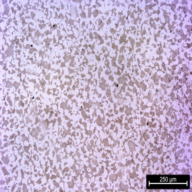
\includegraphics[width=\linewidth]{figures/appendix_preds/4130-steel-viz-original.png} &
        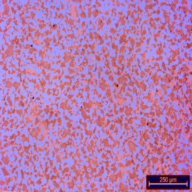
\includegraphics[width=\linewidth]{figures/appendix_preds/4130-steel-viz-mask.png} &
        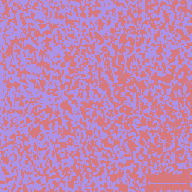
\includegraphics[width=\linewidth]{figures/appendix_preds/4130-steel-pred-classic-rf.png} &
        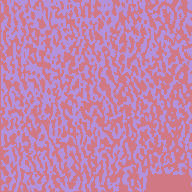
\includegraphics[width=\linewidth]{figures/appendix_preds/4130-steel-pred-deep-unet-effb0.png} &
        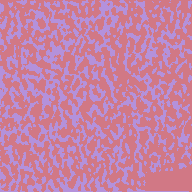
\includegraphics[width=\linewidth]{figures/appendix_preds/4130-steel-pred-metal-unetpp-clahe-effb0.png} \\
        \midrule
        6280 Gray Cast Iron (x10)\\Cast iron | as-cast | x10 &
        Coarse graphite flakes against ferrite matrix stress class imbalance and flake-interface delineation. &
        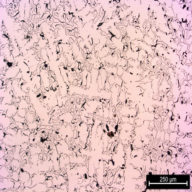
\includegraphics[width=\linewidth]{figures/appendix_preds/6280-cast-iron-low-viz-original.png} &
        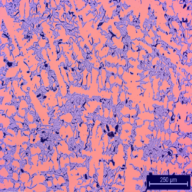
\includegraphics[width=\linewidth]{figures/appendix_preds/6280-cast-iron-low-viz-mask.png} &
        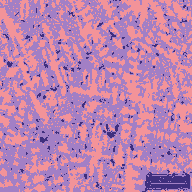
\includegraphics[width=\linewidth]{figures/appendix_preds/6280-cast-iron-low-pred-classic-rf.png} &
        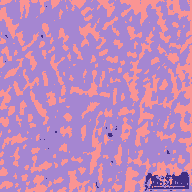
\includegraphics[width=\linewidth]{figures/appendix_preds/6280-cast-iron-low-pred-deep-unet-effb0.png} &
        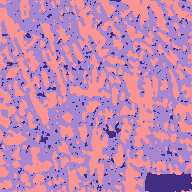
\includegraphics[width=\linewidth]{figures/appendix_preds/6280-cast-iron-low-pred-metal-unetpp-clahe-effb0.png} \\
        \midrule
        6280 Gray Cast Iron (x20)\\Cast iron | as-cast | x20 &
        This x20 example illustrates a scale-dependent morphology shift and
        boundary-fidelity challenge relative to the x10 subset. &
        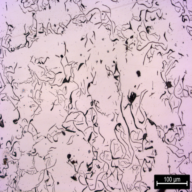
\includegraphics[width=\linewidth]{figures/appendix_preds/6280-cast-iron-high-viz-original.png} &
        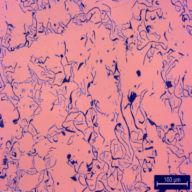
\includegraphics[width=\linewidth]{figures/appendix_preds/6280-cast-iron-high-viz-mask.png} &
        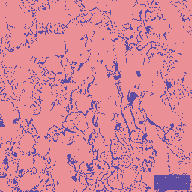
\includegraphics[width=\linewidth]{figures/appendix_preds/6280-cast-iron-high-pred-classic-rf.png} &
        
\includegraphics[width=\linewidth]{figures/appendix_preds/6280-cast-iron-high-pred-deep-unet-effb0.png} &
        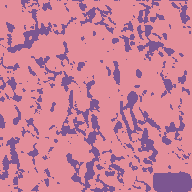
\includegraphics[width=\linewidth]{figures/appendix_preds/6280-cast-iron-high-pred-metal-unetpp-clahe-effb0.png} \\
        \bottomrule
    \end{tabularx}
\end{table*}

\begin{table*}[ht]
    \centering
    \tablefontsize
    \setlength{\tabcolsep}{1.8pt}
    \renewcommand{\arraystretch}{1.06}
    \caption{Expanded representative visual diversity audit (Part II/II): remaining three subsets, using the same aligned layout for multi-scale and printed-alloy stress slices.}
    \label{tab:rep_visual_diversity_part2}
    \begin{tabularx}{\textwidth}{>{\raggedright\arraybackslash}p{0.15\textwidth} >{\raggedright\arraybackslash}X *{5}{>{\centering\arraybackslash}m{0.11\textwidth}}}
        \toprule
        Sample profile & Why this sample matters benchmark-wise & Original & Mask & Classical Rep. & Deep Rep. & Metal Rep. \\
        \midrule
        5884 Armor Steel (x5)\\Steel Q\&T | x5 &
        This x5 example represents a subset that also contains x10/x20/x50 images and highlights ambiguous grain/dendrite boundaries at one scale. &
        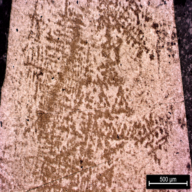
\includegraphics[width=\linewidth]{figures/appendix_preds/5884-armor-steel-viz-original.png} &
        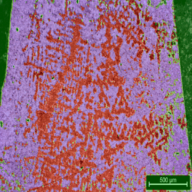
\includegraphics[width=\linewidth]{figures/appendix_preds/5884-armor-steel-viz-mask.png} &
        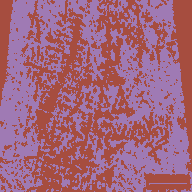
\includegraphics[width=\linewidth]{figures/appendix_preds/5884-armor-steel-pred-classic-rf.png} &
        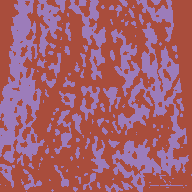
\includegraphics[width=\linewidth]{figures/appendix_preds/5884-armor-steel-pred-deep-unet-effb0.png} &
        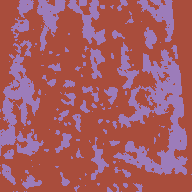
\includegraphics[width=\linewidth]{figures/appendix_preds/5884-armor-steel-pred-metal-unetpp-clahe-effb0.png} \\
        \midrule
        418 Printed 17-4 PH (x5)\\Printed steel | as-sintered | x5 &
        Sparse pores and local inclusions test artifact robustness and false-positive control in phase maps. &
        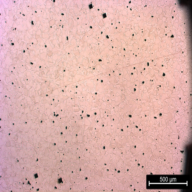
\includegraphics[width=\linewidth]{figures/appendix_preds/418-17-4ph-x5-viz-original.png} &
        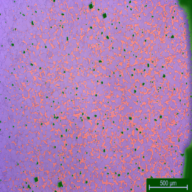
\includegraphics[width=\linewidth]{figures/appendix_preds/418-17-4ph-x5-viz-mask.png} &
        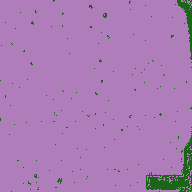
\includegraphics[width=\linewidth]{figures/appendix_preds/418-17-4ph-x5-pred-classic-rf.png} &
        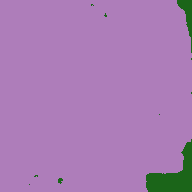
\includegraphics[width=\linewidth]{figures/appendix_preds/418-17-4ph-x5-pred-deep-unet-effb0.png} &
        
\includegraphics[width=\linewidth]{figures/appendix_preds/418-17-4ph-x5-pred-metal-unetpp-clahe-effb0.png} \\
        \midrule
        418 Printed 17-4 PH (x20)\\Printed steel | as-sintered | x20 &
        x20 reshapes pore visibility and texture statistics, illustrating a
        scale-dependent in-corpus challenge. &
        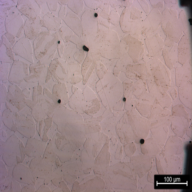
\includegraphics[width=\linewidth]{figures/appendix_preds/418-17-4ph-x20-viz-original.png} &
        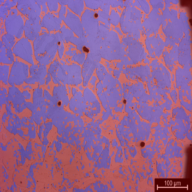
\includegraphics[width=\linewidth]{figures/appendix_preds/418-17-4ph-x20-viz-mask.png} &
        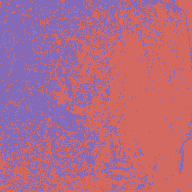
\includegraphics[width=\linewidth]{figures/appendix_preds/418-17-4ph-x20-pred-classic-rf.png} &
        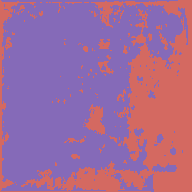
\includegraphics[width=\linewidth]{figures/appendix_preds/418-17-4ph-x20-pred-deep-unet-effb0.png} &
        
\includegraphics[width=\linewidth]{figures/appendix_preds/418-17-4ph-x20-pred-metal-unetpp-clahe-effb0.png} \\
        \bottomrule
    \end{tabularx}
\end{table*}

\section{Release Annotation Notes (Appendix)}\label{app:annotationnotes}
Table~\ref{tab:annotation_notes} summarizes and lightly normalizes the subset
descriptions and annotation notes stored in
\texttt{assets/data/amam-dataset.json}, together
with the pair counts reconstructed from the release. The metadata does not
record the author or reviewer of each individual note, so the table does not
attribute them more specifically.

\textbf{Scope note.} The release manifest lists
\texttt{3105-aluminum-high} and \texttt{7075-aluminum-low} as excluded
subsets. They are therefore outside the strict AMAM-128 evaluation set and do
not appear in Table~\ref{tab:annotation_notes}.

\begin{table*}[ht]
    \centering
    \tablefontsize
    \setlength{\tabcolsep}{3pt}
    \renewcommand{\arraystretch}{1.08}
    \caption{Release-metadata descriptions and annotation notes for the strict
    AMAM-128 subsets.}
    \label{tab:annotation_notes}
    \begin{tabularx}{\textwidth}{>{\raggedright\arraybackslash}p{0.20\textwidth}>{\raggedright\arraybackslash}p{0.16\textwidth}>{\raggedright\arraybackslash}X>{\raggedright\arraybackslash}X>{\centering\arraybackslash}p{0.08\textwidth}}
        \toprule
        Subset & Material / condition & Release description & Release annotation note & Paired tuples \\
        \midrule
        4130 Steel (x10/x20) & Steel; normalized; x10/x20 & Ferrite and pearlite morphology with clear phase contrast. & Ferrite is labeled in blue and pearlite in red; some pores or scratches can be confused with pearlite. & 40 \\
        \midrule
        6280 Gray Cast Iron (x10) & Cast iron; as-cast; x10 & Large ferrite dendrites with an interdendritic region rich in ferrite and graphite flakes. & Dendrites are highlighted in red and the interdendritic area in blue; some low-graphite regions may be misannotated. & 11 \\
        \midrule
        6280 Gray Cast Iron (x20) & Cast iron; as-cast; x20 & High-magnification views resolve the ferrite matrix and graphite flakes. & Thin graphite flakes increase annotation difficulty and may require near pixel-level labeling. & 10 \\
        \midrule
        5884 Armor Steel (x5/x10/x20/x50) & Steel; quenched and tempered; x5/x10/x20/x50 & Etched images reveal pre-austenite grains with challenging blurry boundaries. & Dendrites are marked in red and interdendritic areas in blue; boundary blur can produce small local errors. & 21 \\
        \midrule
        418 Printed 17-4 PH (x5) & Printed steel; as-sintered; x5 & Sintered ferrite particles with subtle contrast between grains and intergranular regions. & The release metadata records good overall annotation quality after iterative training, with occasional difficult regions. & 25 \\
        \midrule
        418 Printed 17-4 PH (x20) & Printed steel; as-sintered; x20 & Higher-magnification printed ferritic morphology includes more difficult local annotation regions. & Some samples remain challenging and can exhibit incomplete segmentation in local areas. & 21 \\
        \bottomrule
    \end{tabularx}
\end{table*}

\section{Model Survey Tables (Appendix)}\label{app:modelsurvey}
No duplicate model-survey table is included here; the canonical 45-method
results are consolidated in Table~\ref{tab:benchmark-model-results}.

\section{Benchmark Website Usage Guide (Appendix)}\label{app:website}
The benchmark repository is available at
\url{https://github.com/Scientific-Computing-Lab/AMAM}. It contains the
companion interactive explorer, aligned subset/mask views, benchmark result
tables, and downloadable artifacts for the same strict pair-only release used
in this paper. These materials improve transparency and qualitative auditing
(sample-level inspection, artifact-focused error review, and access to released
result files), while the canonical full-pair protocol and reporting
requirements remain those defined in the manuscript and protocol manifests.
Table~\ref{tab:website_artifacts} maps each artifact to its practical value for
reproducible benchmarking submissions.

\begin{table}[ht]
    \centering
    \tablefontsize
    \caption{Companion website artifacts and their benchmark-submission relevance.}
    \label{tab:website_artifacts}
    \begin{tabular}{>{\raggedright\arraybackslash}p{0.30\linewidth}>{\raggedright\arraybackslash}p{0.64\linewidth}}
        \toprule
        Website artifact & Submission-relevant value \\
        \midrule
        Subset explorer (\texttt{index.html}) & Makes material/condition/magnification coverage explicit and auditable at sample level. \\
        Aligned image--mask browsing & Supports artifact-focused qualitative analysis (blur, pores, scratches, reflective confounds). \\
        Benchmark result report (\texttt{report.html}) & Exposes model-block comparisons with the same metric schema used in this manuscript. \\
        Released CSV bundles & Support recomputation of the fixed-seed tables and expose both the 145 model--seed deep values and their five-run mIoU summary. \\
        Provenance + consistency audit files & Record model-source identifiers and check internal agreement within the published artifact bundle; they do not demonstrate an independent rerun. \\
        Repository zip + manifest & Provide convenient packaging; an immutable tag or commit plus an external checksum is required to identify a fixed release. \\
        \bottomrule
    \end{tabular}
\end{table}

\section{Reproducibility Details (Appendix)}\label{app:repro}
This appendix documents how the quantitative tables and representative
prediction visualizations were generated. The 45-method audit follows a
full-pair no-holdout design (implementation label:
\texttt{split\_mode = fullset\_no\_holdout}) with strict pair-only inclusion,
a default reporting seed of 17, and track-specific preprocessing. The
classical routines use 256$\times$256 inputs; the canonical deep and
foundation/edge runs use 192$\times$192 inputs. Reference RGB masks are resized
with bilinear interpolation and converted into class indices using seeded
pixel sampling and K-means centroid estimation. Consequently, unless decoded
class maps are frozen across runs, changing the seed can affect both
model-side stochasticity and the evaluation labels themselves.

Eight clustering/edge classical procedures and all foundation/edge methods
emit arbitrary segment identifiers. The RF/SVM pixel learners emit decoded
class identifiers, but the executed evaluator nevertheless applies
\emph{per-image} Hungarian alignment to every classical and foundation/edge
prediction, using the reference mask and known subset phase count. Their scores
therefore measure partition overlap under oracle label-permutation matching
rather than end-to-end semantic label assignment. Supervised deep models use
the known subset-valid output classes but predict decoded class identifiers
directly and receive no Hungarian alignment. Thus, although all tracks share
the paired corpus and subset-macro aggregation, their prediction-to-label
handling is track-specific.

Metrics are first computed per image over all $k$ classes declared for that
subset. The implementation assigns IoU and Dice equal to 1 when a class is
absent from both the prediction and reference for an image. Image metrics are
then averaged within each subset, and the six subset means receive equal
weight in the reported subset-macro score. This aggregation prevents the
largest subset from dominating, but the absent-class convention can reward
images that omit rare classes and must be kept fixed in future comparisons.

The classical and foundation/edge columns in
Table~\ref{tab:benchmark-model-results} are seed-17 point estimates; the
canonical release does not attach a cross-seed uncertainty estimate to either
track. The deep track was executed as five clean, non-resumed retraining runs
(seeds 17--21), each in a separate output directory. The seed controls
initialization, batch order, augmentation, sampling, centroid estimation, and
label decoding. The resulting per-model mIoU mean, sample standard deviation,
observed range, and rank range are published in
\texttt{repro/results/deep\_survey\_multiseed\_summary.csv}. The tracked
release also contains the 145 model--seed values in
\texttt{repro/results/deep\_survey\_multiseed\_runs.csv} and the aggregation
code in \texttt{repro/benchmark/aggregate\_deep\_multiseed.py}. The
RF/SVM pixel learners and supervised deep variants are fit on all
\paircount{} tuples and reported on those same tuples; foundation/edge add-ons
do not update pretrained network weights from AMAM labels, although their
downstream clustering and post-processing are data-adaptive.

Seed-17 per-image, per-subset, and aggregate outputs are in
\texttt{repro/results/classical/benchmark\_*.csv},
\texttt{repro/results/deep\_survey/deep\_*.csv}, and
\texttt{repro/results/foundation\_edge/foundation\_edge\_*.csv}. Campaign
traceability artifacts are
\texttt{repro/results/model\_provenance\_manifest.csv} and
\texttt{repro/results/reproducibility\_audit\_45\_models.json}; the latter
checks the published artifact bundle (model counts, cross-file agreement,
five-run deep aggregation, and artifact hashes) and is not an independent
rerun test.
It should be regenerated from the final release commit before publication.


\section{Reporting and Validity Notes (Appendix)}\label{app:validity}
\textbf{Recommended reporting minimum.} For comparable submissions, we
recommend publishing: (i) subset-macro mIoU as the primary score, with the
exact image-to-subset-to-global aggregation rule; (ii) per-subset metrics and
confusion matrices; (iii) immutable dataset-release and evaluation-protocol
identifiers and hashes; (iv) individual run values plus the mean and sample
standard deviation over at least three independent clean end-to-end runs for
every pipeline containing stochastic training, sampling, clustering, label
decoding, inference, or post-processing; and (v) complete disclosure of
resizing and interpolation, preprocessing, valid-class restriction,
absent-class scoring, and any label-alignment procedure. Seeds, hardware,
software versions, code revision, and pretrained-checkpoint identity should
accompany these results. Run-to-run standard deviation is not a confidence
interval for dataset-sampling uncertainty; the latter requires separate
image- or subset-aware resampling.

\textbf{Coverage in this release.} The executed five-run deep experiment
reports the individual model--seed mIoU values together with their mean,
sample standard deviation, range, and rank range. Classical and
foundation/edge results remain seed-17 point estimates. Thus, uncertainty
statements in this paper apply to the executed deep pipeline, not automatically
to the other tracks or to dataset sampling.

\textbf{Known limitations.} AMAM-128 is intentionally strict but compact.
Several subsets are small, including 6280 Gray Cast Iron x20 ($n=10$) and x10
($n=11$). The six subset-native label spaces comprise 13 local class slots but
only nine distinct phase names; they are not globally unified.
The executed campaign uses a full-pair no-holdout protocol, so its scores are
in-corpus diagnostics rather than estimates of out-of-sample generalization.
Classical and foundation/edge segment identifiers are aligned to reference
classes separately for each image using the known phase count and Hungarian
assignment; their scores therefore measure partition overlap under oracle
label permutation. Deep predictions do not receive that alignment. Moreover,
the evaluator bilinearly resizes RGB masks and decodes them with seeded
sampling and K-means centroids. Unless those label maps are frozen across runs,
multi-seed statistics quantify end-to-end pipeline variability rather than
model-only variability. The absent-class convention gives a perfect
per-image class score when both maps omit a class. The present release also
lacks a held-out protocol, dataset-sampling confidence intervals, released
per-subset confusion matrices, and a quantified inter-annotator analysis.

\textbf{Threats to validity.} Even with strict pair filtering and
protocol-controlled, seeded preprocessing, several risks remain for
leaderboard-style claims. \emph{Release and protocol drift}: benchmark
conclusions can change if tuple membership, label definitions, preprocessing,
or evaluation mappings change without a new release identifier and manifest
hash. \emph{Implementation and environment drift}: dependency, checkpoint,
hardware, and numerical-kernel changes can alter outputs even under a fixed
seed. \emph{Subset-size imbalance}: small slices produce less stable subset
estimates and can amplify changes in subset-macro rankings.
\emph{Oracle-alignment optimism}: using the reference mask to permute labels
per image can overstate end-to-end semantic performance and prevents strict
cross-track rank interpretation. \emph{Stochastic-pipeline variation}: score
differences that are small relative to observed run-to-run spread warrant
caution and should not support fine-grained ordering without a prespecified
paired analysis.
\emph{No-split optimism}: methods fitted and evaluated on the same tuples can
overestimate deployment performance. Accordingly, per-subset metrics,
confusion matrices, and run-to-run summaries should be treated as first-class
outputs. Confidence intervals for
dataset-sampling uncertainty, when reported, should be computed separately
using image- or subset-aware resampling.

\textbf{Submission packet template.} To keep reported gains auditable, we
recommend each benchmark submission include the following artifacts:
\begin{enumerate}[leftmargin=*,nosep]
    \item immutable dataset tag or commit, dataset-manifest hash, and
    evaluation-protocol hash;
    \item code revision, model architecture, initialization source, and exact
    pretrained-checkpoint identity;
    \item input and label-pipeline configuration, including resize size and
    interpolation, augmentation, preprocessing, valid classes, missing-class
    handling, and prediction-to-label alignment;
    \item individual per-run metrics and a summary reporting mean, sample
    standard deviation, observed score range, and rank range over at least
    three clean runs for stochastic pipelines;
    \item per-subset metrics and confusion matrices, with any confidence
    interval for dataset-sampling uncertainty computed and labeled separately;
    \item compute disclosure (GPU/CPU type, software environment, wall-clock
    training and inference time, and parameter count).
\end{enumerate}
These requirements provide a practical baseline for auditable comparison
across submissions.

\end{document}
